\documentclass{article}
\usepackage[margin = 1in]{geometry}
\usepackage{graphicx}
\usepackage{amsmath}
\usepackage{amssymb}
\usepackage{bm}
\usepackage{tcolorbox}
\usepackage{latex-rmd}
\newcommand{\E}{\mathrm{E}}
\newcommand{\Log}{\log}
\renewcommand{\log}{\:\mathrm{log}\:}
\renewcommand\thesubsection{\thesection.\alph{subsection}}
\setlength{\parindent}{0em}
\setlength{\parskip}{1em}

\title{Advanced Macroeconometrics - Assignment 2}
\author{Miriam Frauenlob, Elisabeth Fidrmuc, Tim Koenders }
\date{May 2023}

\begin{document}

\maketitle

\vspace{2em}

\begin{tcolorbox}
\centering \itshape The executable code that was used in compiling the assignment is available on GitHub at \href{https://github.com/TimKoenders/macrometrics2}{https://github.com/TimKoenders/macrometrics2}.
\end{tcolorbox}

\newpage


\section*{Question 1}

\vspace{2em}

\begin{center}
\textbf{Simulating draws from a Normal distribution and estimating the mean} 
\end{center}

\vspace{2em}

\begin{Shaded}
\begin{Highlighting}[]
\NormalTok{knitr}\SpecialCharTok{::}\NormalTok{opts\_chunk}\SpecialCharTok{$}\FunctionTok{set}\NormalTok{(}\AttributeTok{fig.width=}\DecValTok{12}\NormalTok{, }\AttributeTok{fig.height=}\DecValTok{8}\NormalTok{, }\AttributeTok{fig\_path=}\StringTok{\textquotesingle{}figures/\textquotesingle{}}\NormalTok{,}\AttributeTok{echo=}\ConstantTok{TRUE}\NormalTok{, }\AttributeTok{warning=}\ConstantTok{FALSE}\NormalTok{, }\AttributeTok{message=}\ConstantTok{FALSE}\NormalTok{)}

\CommentTok{\# Define parameters}
\NormalTok{mu }\OtherTok{\textless{}{-}} \DecValTok{5}
\NormalTok{sigma }\OtherTok{\textless{}{-}} \DecValTok{9}
\NormalTok{n }\OtherTok{\textless{}{-}} \DecValTok{100}

\CommentTok{\# Generate data}
\NormalTok{x }\OtherTok{\textless{}{-}} \FunctionTok{rnorm}\NormalTok{(n, }\AttributeTok{mean =}\NormalTok{ mu, }\AttributeTok{sd =}\NormalTok{ sigma)}

\CommentTok{\# Compute estimates of the mean with the first 1, ..., n draws}
\NormalTok{estimates }\OtherTok{\textless{}{-}} \FunctionTok{cumsum}\NormalTok{(x) }\SpecialCharTok{/} \FunctionTok{seq\_along}\NormalTok{(x)}

\CommentTok{\# Plot estimates}
\FunctionTok{plot}\NormalTok{(estimates, }\AttributeTok{type =} \StringTok{"l"}\NormalTok{, }\AttributeTok{col =} \StringTok{"blue"}\NormalTok{, }\AttributeTok{xlab =} \StringTok{"Sample size"}\NormalTok{, }\AttributeTok{ylab =} \StringTok{"Estimate of the mean"}\NormalTok{)}

\CommentTok{\# Add true mean as a horizontal line}
\FunctionTok{abline}\NormalTok{(}\AttributeTok{h =}\NormalTok{ mu, }\AttributeTok{col =} \StringTok{"red"}\NormalTok{)}
\end{Highlighting}
\end{Shaded}


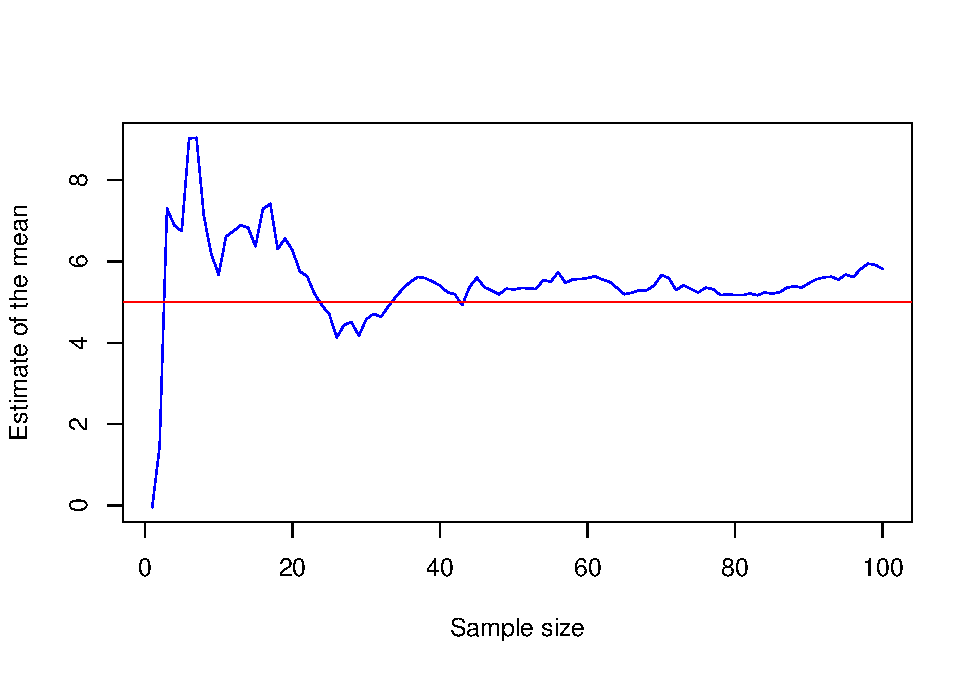
\includegraphics{Figures and Plots/figure-latex/global_options2-1.pdf}
The plot below highlights the law of large numbers in action, where increasing
the sample size results in estimates of the mean that converge to the
true mean. While initial estimates may deviate from the true mean, as
the sample size increases, the estimates become more stable and approach
the true mean with greater precision.


\begin{center}
\textbf{Simulating draws from a Cauchy distribution and estimating the mean} 
\end{center}

\vspace{2em}


\begin{Shaded}
\begin{Highlighting}[]
\NormalTok{knitr}\SpecialCharTok{::}\NormalTok{opts\_chunk}\SpecialCharTok{$}\FunctionTok{set}\NormalTok{(}\AttributeTok{fig.width=}\DecValTok{12}\NormalTok{, }\AttributeTok{fig.height=}\DecValTok{8}\NormalTok{, }\AttributeTok{fig\_path=}\StringTok{\textquotesingle{}figures/\textquotesingle{}}\NormalTok{,}\AttributeTok{echo=}\ConstantTok{TRUE}\NormalTok{, }\AttributeTok{warning=}\ConstantTok{FALSE}\NormalTok{, }\AttributeTok{message=}\ConstantTok{FALSE}\NormalTok{)}

\CommentTok{\# Define parameters}
\NormalTok{mu }\OtherTok{\textless{}{-}} \DecValTok{0}
\NormalTok{sigma }\OtherTok{\textless{}{-}} \DecValTok{1}
\NormalTok{n }\OtherTok{\textless{}{-}} \DecValTok{1000}

\CommentTok{\# Generate two random samples from a standard normal distribution}
\NormalTok{x }\OtherTok{\textless{}{-}} \FunctionTok{rnorm}\NormalTok{(n, }\AttributeTok{mean =}\NormalTok{ mu, }\AttributeTok{sd =}\NormalTok{ sigma)}
\NormalTok{y }\OtherTok{\textless{}{-}} \FunctionTok{rnorm}\NormalTok{(n, }\AttributeTok{mean =}\NormalTok{ mu, }\AttributeTok{sd =}\NormalTok{ sigma)}

\CommentTok{\# Convert the standard normal samples to a Cauchy distribution with scale one}
\NormalTok{z }\OtherTok{\textless{}{-}}\NormalTok{ x }\SpecialCharTok{/}\NormalTok{ y}

\CommentTok{\# Compute estimates of the mean with the first 1, ..., n draws}
\NormalTok{estimates }\OtherTok{\textless{}{-}} \FunctionTok{cumsum}\NormalTok{(z) }\SpecialCharTok{/} \FunctionTok{seq\_along}\NormalTok{(z)}

\CommentTok{\# Plot estimates}
\FunctionTok{plot}\NormalTok{(estimates, }\AttributeTok{type =} \StringTok{"l"}\NormalTok{, }\AttributeTok{col =} \StringTok{"blue"}\NormalTok{, }\AttributeTok{xlab =} \StringTok{"Sample size"}\NormalTok{, }\AttributeTok{ylab =} \StringTok{"Estimate of the mean"}\NormalTok{)}

\CommentTok{\# Add true mean as a horizontal line}
\FunctionTok{abline}\NormalTok{(}\AttributeTok{h =}\NormalTok{ mu, }\AttributeTok{col =} \StringTok{"red"}\NormalTok{)}
\end{Highlighting}
\end{Shaded}

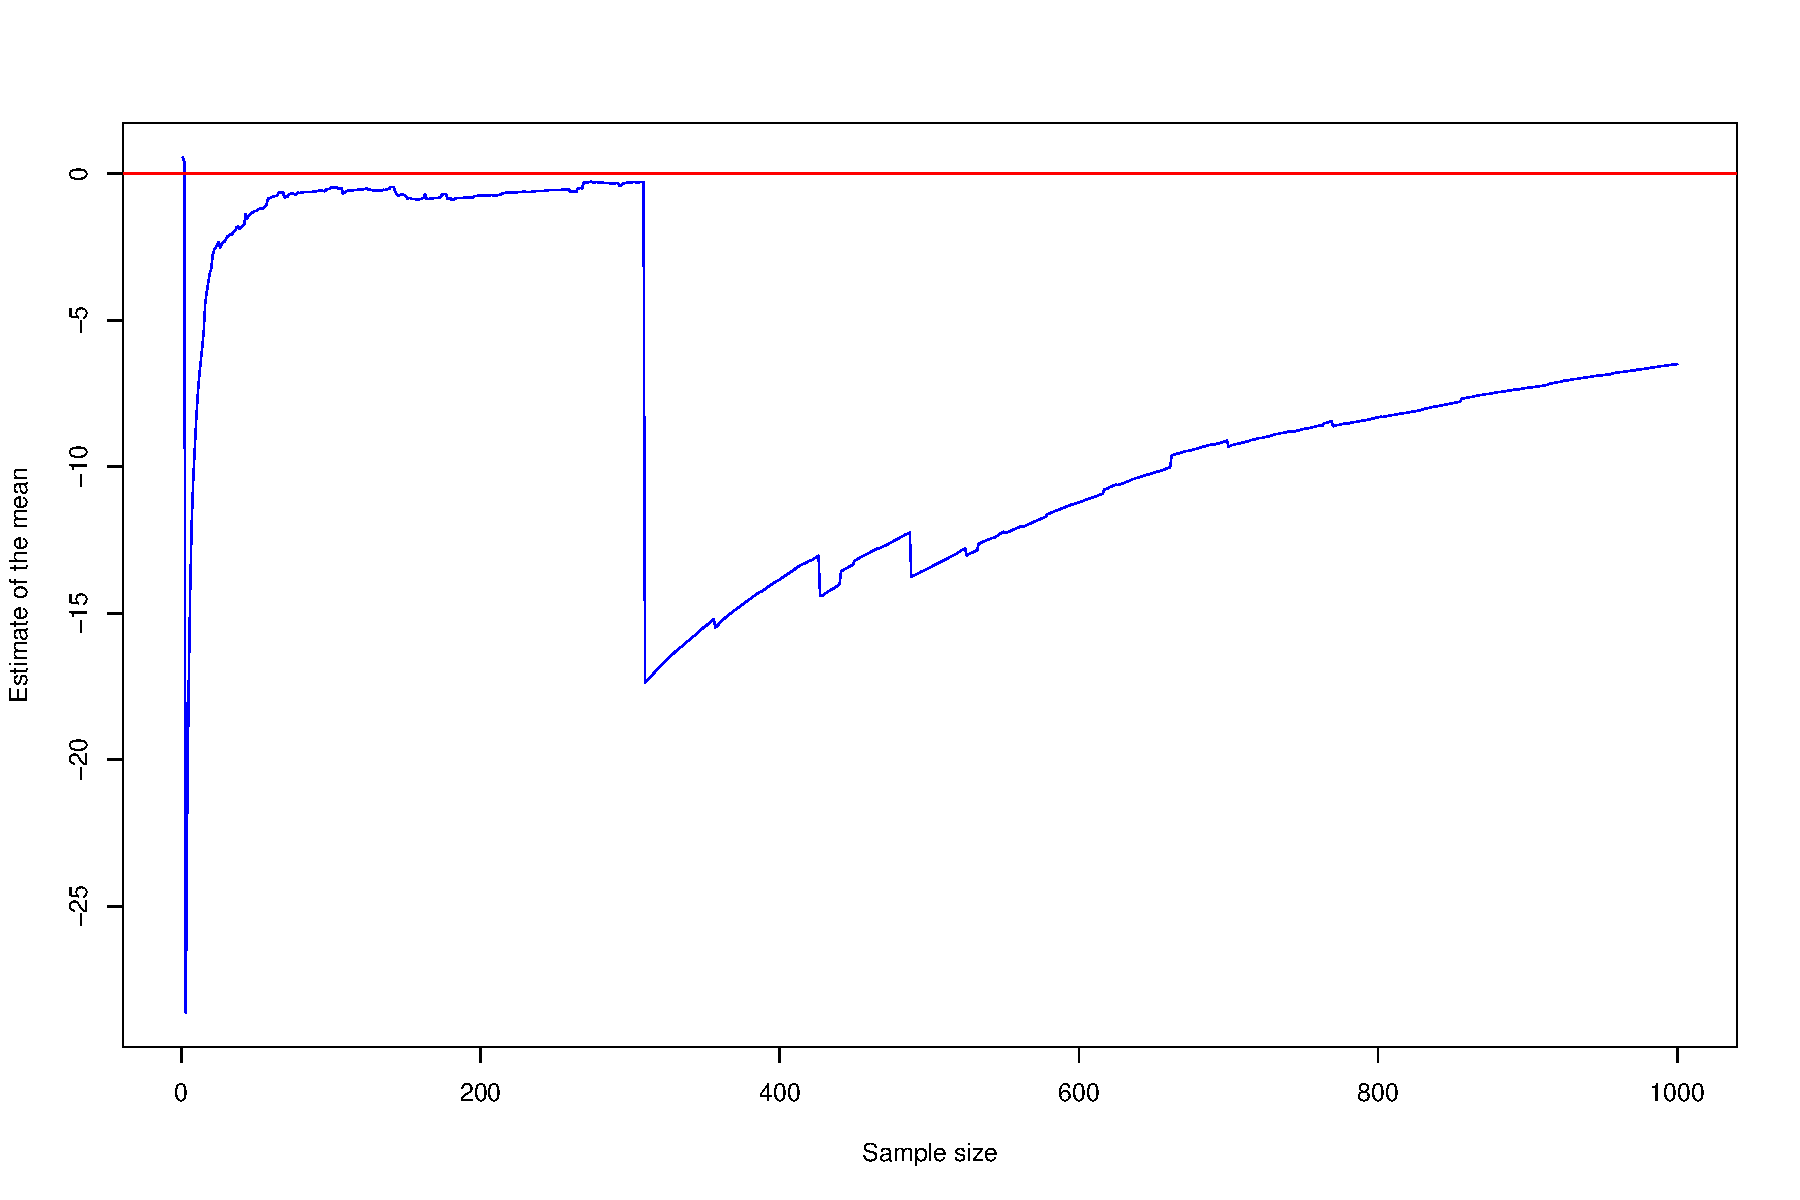
\includegraphics{Figures and Plots/figure-latex/global_options3-1.pdf}
\newpage 

The plot generated by the code shows the estimates of the mean of a
Cauchy distribution with increasing sample sizes. The blue line
represents the estimated mean and the red line represents the true mean, which is zero in this case. The Cauchy
distribution does not have a well-defined expectation as the improper integral $\displaystyle \int_{-\infty}^{\infty} \frac{x}{\pi(1+x^2)} \, dx$ diverges. This means that the distribution does not converge
to a particular value as the sample size increases.

\section*{Question 2}

\vspace{2em}

\begin{center}
\textbf{What is the class of conjugate priors? Derive the posterior distribution} 
\end{center}

\vspace{2em}

Because we can model the Covid tests with a Bernoulli distribution, the class of conjugate priors is the Beta distribution. \par
To model the posterior distribution, we start with specifying the prior as \par
\begin{center}
  $p(\theta) \sim \operatorname{Beta}(a_{0}, b_{0})$   
\end{center}

\par 
We know that the posterior distribution is proportional to the product of the prior distribution and the likelihood:
\begin{center}
$p(\theta \mid y) \propto p(y \mid \theta) p(\theta)$
\end{center}

where $S=\sum_{i=1}^{n}y_{i}$ is the number of positive tests.

Because we have Bernoulli trials, the likelihood function is the following: \par 
\begin{center}
    $p(y \mid \theta) = \theta^S (1 - \theta)^{n-S}$
\end{center}

where $n$ is the number of observations and $n-S$ is the number of negative tests.

Through Bayes theorem we get the normalized posterior distribution \par 
\begin{center}
    $p(\theta \mid y) = \frac{p(y \mid \theta) p(\theta)}{p(y)}$
    \end{center}
The posterior distribution is proportional to the product of the likelihood and the prior distribution. Inserting the prior and likelihood yields \par 
\begin{center}
    $p(\theta \mid y) \propto \theta^S (1 - \theta)^{n-S} \theta^{(a_{0}-1} (1 - \theta)^{b_{0}-1}$ \\
    $p(\theta \mid y) \propto \theta^{S+a_{0}-1} (1 - \theta)^{n-S+b_{0}-1}$ \\
    $p(\theta \mid y) \propto \theta^{a_{n}-1} (1 - \theta)^{b_{n}-1}$

\end{center}

where $a_{n}=S+a_{0}$ and $b_{n}=n-S+b_{0}$.

It becomes clear that the posterior follows a Beta distribution. \par 
\begin{center}
    $p(\theta \mid y) \propto \operatorname{Beta}(a_{n}, b_{n})$ \par
    
\newpage

\end{center}
\begin{center}
 \textbf{Assume you have observations for thirty days (n= 30) with a total of ten positive tests. Determine and briefly explain several point estimators of $\theta$ }
\end{center}

\vspace{2em}

\textit{Bayesian estimators}

With $S=10$ and $n=30$, we know that our posterior follows the Beta distribution $Beta(10+\alpha,20+\beta)$. We could obtain posterior moments (eg. mean or standard deviation), posterior quantiles (eg. median) and many more.

\begin{align*}
    E[\theta]= \frac{a_{n}}{a_n+b_n} \\
    = \frac{10+a_0}{30+a_0+b_0} \\
    V(\theta)=\frac{E[\theta](1-E[\theta])}{a_n+b_n+1}
\end{align*}

The question remains how to choose appropriate priors $a_0$ and $b_0$. We could use an uninformative prior with $a_0=1$ and $b_0=1$ such that $E[\theta]=\frac{a_{0}}{a_0+b_0}=0.5$. We then obtain 

\begin{align*}
    E[\theta]= \frac{10+1}{30+1+1}=0.34 \\
    V(\theta)=\frac{0.34(0.44)}{11+21+1}=0.007
\end{align*}

However, a credible region would be much more informative than a mere point estimate. 


We begin with a Bayesian estimator. As we have shown above, the conjugate prior for our example follows a Beta distribution. For convinience, we choose a Beta (1,1) distribution. We know that our posterior mean of $\theta$ is 
\begin{center}
    $E(\theta \mid y) = \frac{\alpha + S}{\alpha + \beta + n}$
\end{center}
Because the Beta(1,1) distribution is uniform over [0,1], we get the following value for our point estimate for the posterior mean:
\begin{center}
    $(1+10)/(1+20)=0.48.$
\end{center}
Another point estimate we could use would be the mean of our posterior distribution. In our case, this would mean 
\begin{center}
$\frac{an}{an+bn}$\par
$an=a0+Sn=1+10=11$ \par
$bn=b0+n-Sn=1+20-10=11$\par
$ \frac{an}{an+bn}=0.5$
\end{center}
This would mean that we would expect every second Covid test to be positive. \par
\newpage
\textit {Maximum likelihood estimator} \par 
Another point estimate of $\theta$ could be determined using the MLE. We have the following likelihood function:
\begin{center}
    $p(y \mid \theta) = \theta^S (1 - \theta)^{n-S}$
\end{center}
If we set the derivative of the log-likelihood function with respect to $\theta$ 0, we arrive at 
\begin{center}
    $\theta=\frac{S}{n}=\frac{10}{30}=0.33$
\end{center}
\vspace{2em}

\begin{center}
    \textbf{Discuss sources of prior information for this problem and compare the impact of different priors on your point estimates}
\end{center}

\vspace{2em}

Sources of prior information for this problem could come be determined through various ways. First of all, we could have historical information. Maybe we know how many positive Covid tests we on average had in the office throughout a relevant time period.
Further, we could have data on the prevalence of Covid19 in Austria for the relevant time period.
Another source of information might be other scientific estimates about the spread of Covid19.
Additional information on the colleagues could be useful as well. Depending on their vaccination status or if they have previously been infected, their risk of new infection might be different. We could also compare our workplace to a similar one. Say we work at a school, we can obtain information on the prevalence of the disease of a different school with a similar size.
The different sources of prior information affect our estimates depending on how well the prior aligns with the data. If we choose a prior that is too low, then our estimates might be torn towards a lower estimate than actually present in our sample and vice versa. We must, however, note, that clearly only the Bayesian point estimates are influenced by prior information. \par

Below we display the distribution of several potential priors. They are very different. Setting $a_0=b_0=1$ feigns ignorance, ie. we then assume equal probabilty for all outcomes.

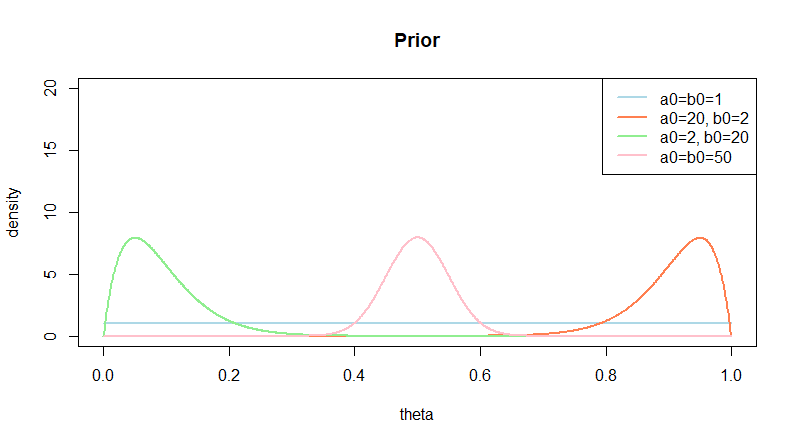
\includegraphics{Figures and Plots/figure-latex/Rplot 2 prior.png}
\newpage
Interestingly, the posterior distributions compared to the prior distributions. It seems that the data pushes the posterior towards a certain outcome, regardless of the prior. The posterior resulting from the "ignorant" prior looks surprisingly good. 

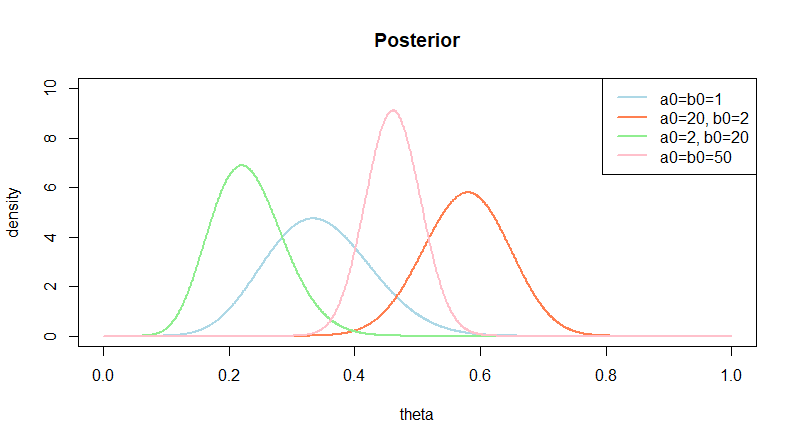
\includegraphics{Figures and Plots/figure-latex/Rplot 2 posterior.png}

It seems that a higher $a_0$ pushes the posterior distribution to the right whilst a higher $b_0$ pushes it to the left. 

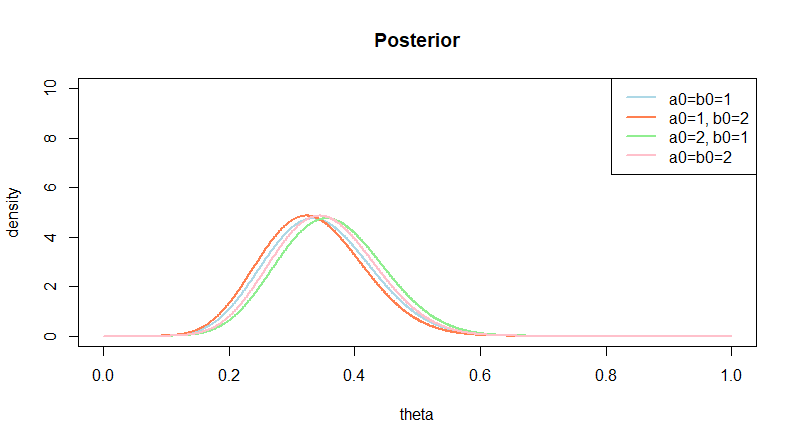
\includegraphics{Figures and Plots/figure-latex/Rplot 2 parameters.png}

\newpage
\begin{center}
    \textbf{Discuss the assumption of independent and identically distributed data. How could you (conceptually)
improve the model with this in mind?
}
\end{center}

\vspace{2em}

The assumption of independent and identically distributed data is debatable if not even controversial when talking about a contagious disease. This lies in the fact that Covid19, like every infectious disease spreads when people meet and as in the office, people meet, chances are high that we might run into a cluster in the office. In this case, the assumption of independence would not hold anymore. For a large number of positive tests, we can expect the number to remain high in the following period 1) since new people could have been infected and 2) as people remain positive for about a week once infected.  \par 

To improve the model, we could assume a time series context where yesterday's results might be indicative of today's results. \par 
Another problem we could run into might be that the assumption of identically distributed data would not hold if the chances of the colleagues getting Covid strongly differs. This might be due to lifestyle or differences in familiar exposure. Also, during lock-downs when home office is enforced for instance, the prevalence of the disease would be much lower. One solution to this problem might be choosing a mixture model with different subgroups. 


\section*{Question 3}
\vspace{2em}

\begin{center}
\textbf{Writing the R function} 
\end{center}
\vspace{2em}

\begin{Shaded}
\begin{Highlighting}[]
\NormalTok{knitr}\SpecialCharTok{::}\NormalTok{opts\_chunk}\SpecialCharTok{$}\FunctionTok{set}\NormalTok{(}\AttributeTok{fig.width=}\DecValTok{12}\NormalTok{, }\AttributeTok{fig.height=}\DecValTok{8}\NormalTok{, }\AttributeTok{fig\_path=}\StringTok{\textquotesingle{}figures/\textquotesingle{}}\NormalTok{,}\AttributeTok{echo=}\ConstantTok{TRUE}\NormalTok{, }\AttributeTok{warning=}\ConstantTok{FALSE}\NormalTok{, }\AttributeTok{message=}\ConstantTok{FALSE}\NormalTok{)}

\FunctionTok{set.seed}\NormalTok{(}\DecValTok{123}\NormalTok{)}

\NormalTok{simulate\_data }\OtherTok{\textless{}{-}} \ControlFlowTok{function}\NormalTok{(n, k, alpha, beta, sigma) \{}
\NormalTok{  X }\OtherTok{\textless{}{-}} \FunctionTok{matrix}\NormalTok{(}\FunctionTok{rnorm}\NormalTok{(n }\SpecialCharTok{*}\NormalTok{ k, }\AttributeTok{mean =} \DecValTok{0}\NormalTok{, }\AttributeTok{sd =} \DecValTok{1}\NormalTok{), n, k)}
\NormalTok{  epsilon }\OtherTok{\textless{}{-}} \FunctionTok{rnorm}\NormalTok{(n, }\AttributeTok{mean =} \DecValTok{0}\NormalTok{, }\AttributeTok{sd =}\NormalTok{ sigma)}
\NormalTok{  y }\OtherTok{\textless{}{-}}\NormalTok{ alpha }\SpecialCharTok{+}\NormalTok{ X }\SpecialCharTok{\%*\%}\NormalTok{ beta }\SpecialCharTok{+}\NormalTok{ epsilon}
  \FunctionTok{return}\NormalTok{(}\FunctionTok{list}\NormalTok{(}\AttributeTok{X =}\NormalTok{ X, }\AttributeTok{y =}\NormalTok{ y))}
\NormalTok{\}}
\end{Highlighting}
\end{Shaded}


\begin{center}
\textbf{Simulating data with k = 1 and $\sigma$ = 1 and plot the x and y in a scatterplot}
\end{center}
\vspace{2em}


\begin{Shaded}
\begin{Highlighting}[]
\NormalTok{knitr}\SpecialCharTok{::}\NormalTok{opts\_chunk}\SpecialCharTok{$}\FunctionTok{set}\NormalTok{(}\AttributeTok{fig.width=}\DecValTok{12}\NormalTok{, }\AttributeTok{fig.height=}\DecValTok{8}\NormalTok{, }\AttributeTok{fig\_path=}\StringTok{\textquotesingle{}figures/\textquotesingle{}}\NormalTok{,}\AttributeTok{echo=}\ConstantTok{TRUE}\NormalTok{, }\AttributeTok{warning=}\ConstantTok{FALSE}\NormalTok{, }\AttributeTok{message=}\ConstantTok{FALSE}\NormalTok{)}

\FunctionTok{set.seed}\NormalTok{(}\DecValTok{123}\NormalTok{)}

\CommentTok{\# Create scatterplot with regression line}
\NormalTok{sim\_data\_1 }\OtherTok{\textless{}{-}} \FunctionTok{sim\_linear\_model\_1}\NormalTok{(}\AttributeTok{n =} \DecValTok{100}\NormalTok{, }\AttributeTok{k =} \DecValTok{1}\NormalTok{, }\AttributeTok{alpha =} \DecValTok{2}\NormalTok{, }\AttributeTok{beta =} \DecValTok{3}\NormalTok{, }\AttributeTok{sigma =} \DecValTok{1}\NormalTok{)}
\FunctionTok{plot}\NormalTok{(sim\_data\_1}\SpecialCharTok{$}\NormalTok{x, sim\_data\_1}\SpecialCharTok{$}\NormalTok{y, }\AttributeTok{xlab =} \StringTok{"x"}\NormalTok{, }\AttributeTok{ylab =} \StringTok{"y"}\NormalTok{)}
\FunctionTok{abline}\NormalTok{(}\FunctionTok{lm}\NormalTok{(y }\SpecialCharTok{\textasciitilde{}}\NormalTok{ x, }\AttributeTok{data =}\NormalTok{ sim\_data\_1), }\AttributeTok{col =} \StringTok{"red"}\NormalTok{)}
\end{Highlighting}
\end{Shaded}

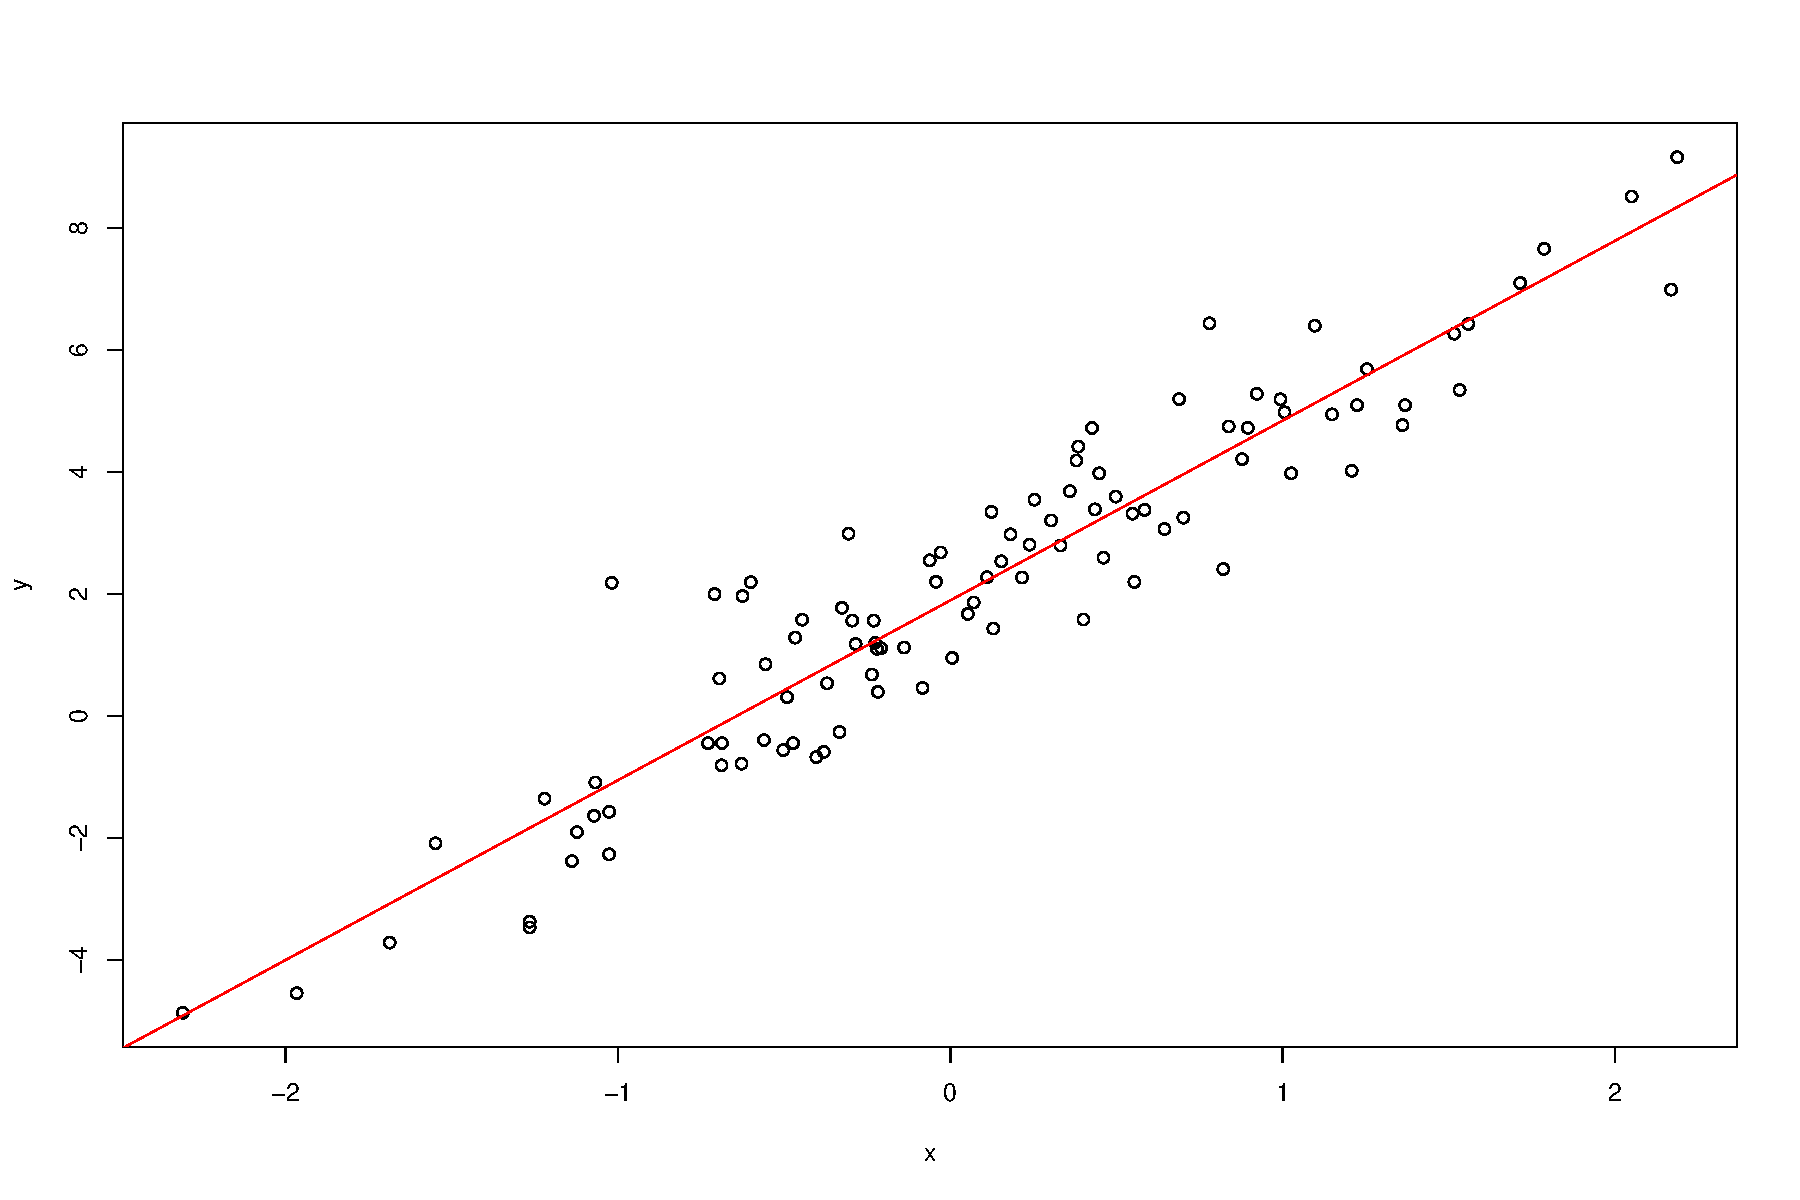
\includegraphics{Figures and Plots/figure-latex/global_options4-1.pdf}



\begin{center}
\textbf{Simulating data 1000 times and create histogram of estimates}
\end{center}

\vspace{2em}

\begin{Shaded}
\begin{Highlighting}[]
\CommentTok{\# Define numbers of simulations}

\NormalTok{n\_sims }\OtherTok{\textless{}{-}} \DecValTok{1000}

\CommentTok{\# Create an empty vector to store the estimated slope coefficients}
\NormalTok{beta\_lse }\OtherTok{\textless{}{-}} \FunctionTok{numeric}\NormalTok{(n\_sims)}

\CommentTok{\# Loop through the simulations}
\ControlFlowTok{for}\NormalTok{ (i }\ControlFlowTok{in} \DecValTok{1}\SpecialCharTok{:}\NormalTok{n\_sims) \{}
  \CommentTok{\# Simulate the data}
\NormalTok{  sim\_data\_1 }\OtherTok{\textless{}{-}} \FunctionTok{sim\_linear\_model\_1}\NormalTok{(}\AttributeTok{n =} \DecValTok{100}\NormalTok{, }\AttributeTok{k =} \DecValTok{1}\NormalTok{, }\AttributeTok{alpha =} \DecValTok{2}\NormalTok{, }\AttributeTok{beta =} \DecValTok{3}\NormalTok{, }\AttributeTok{sigma =} \DecValTok{1}\NormalTok{)}
  
  \CommentTok{\# Estimate the slope coefficient using linear regression}
\NormalTok{  fit }\OtherTok{\textless{}{-}} \FunctionTok{lm}\NormalTok{(sim\_data\_1}\SpecialCharTok{$}\NormalTok{y }\SpecialCharTok{\textasciitilde{}}\NormalTok{ sim\_data\_1}\SpecialCharTok{$}\NormalTok{x)}
\NormalTok{  beta\_lse[i] }\OtherTok{\textless{}{-}} \FunctionTok{coef}\NormalTok{(fit)[}\DecValTok{2}\NormalTok{]}
\NormalTok{\}}

\CommentTok{\# Creating histogram}
\FunctionTok{hist}\NormalTok{(beta\_lse, }\AttributeTok{main =} \StringTok{"Histogram of Beta Estimates"}\NormalTok{, }\AttributeTok{xlab =} \StringTok{"Beta Estimate"}\NormalTok{)}
\end{Highlighting}
\end{Shaded}


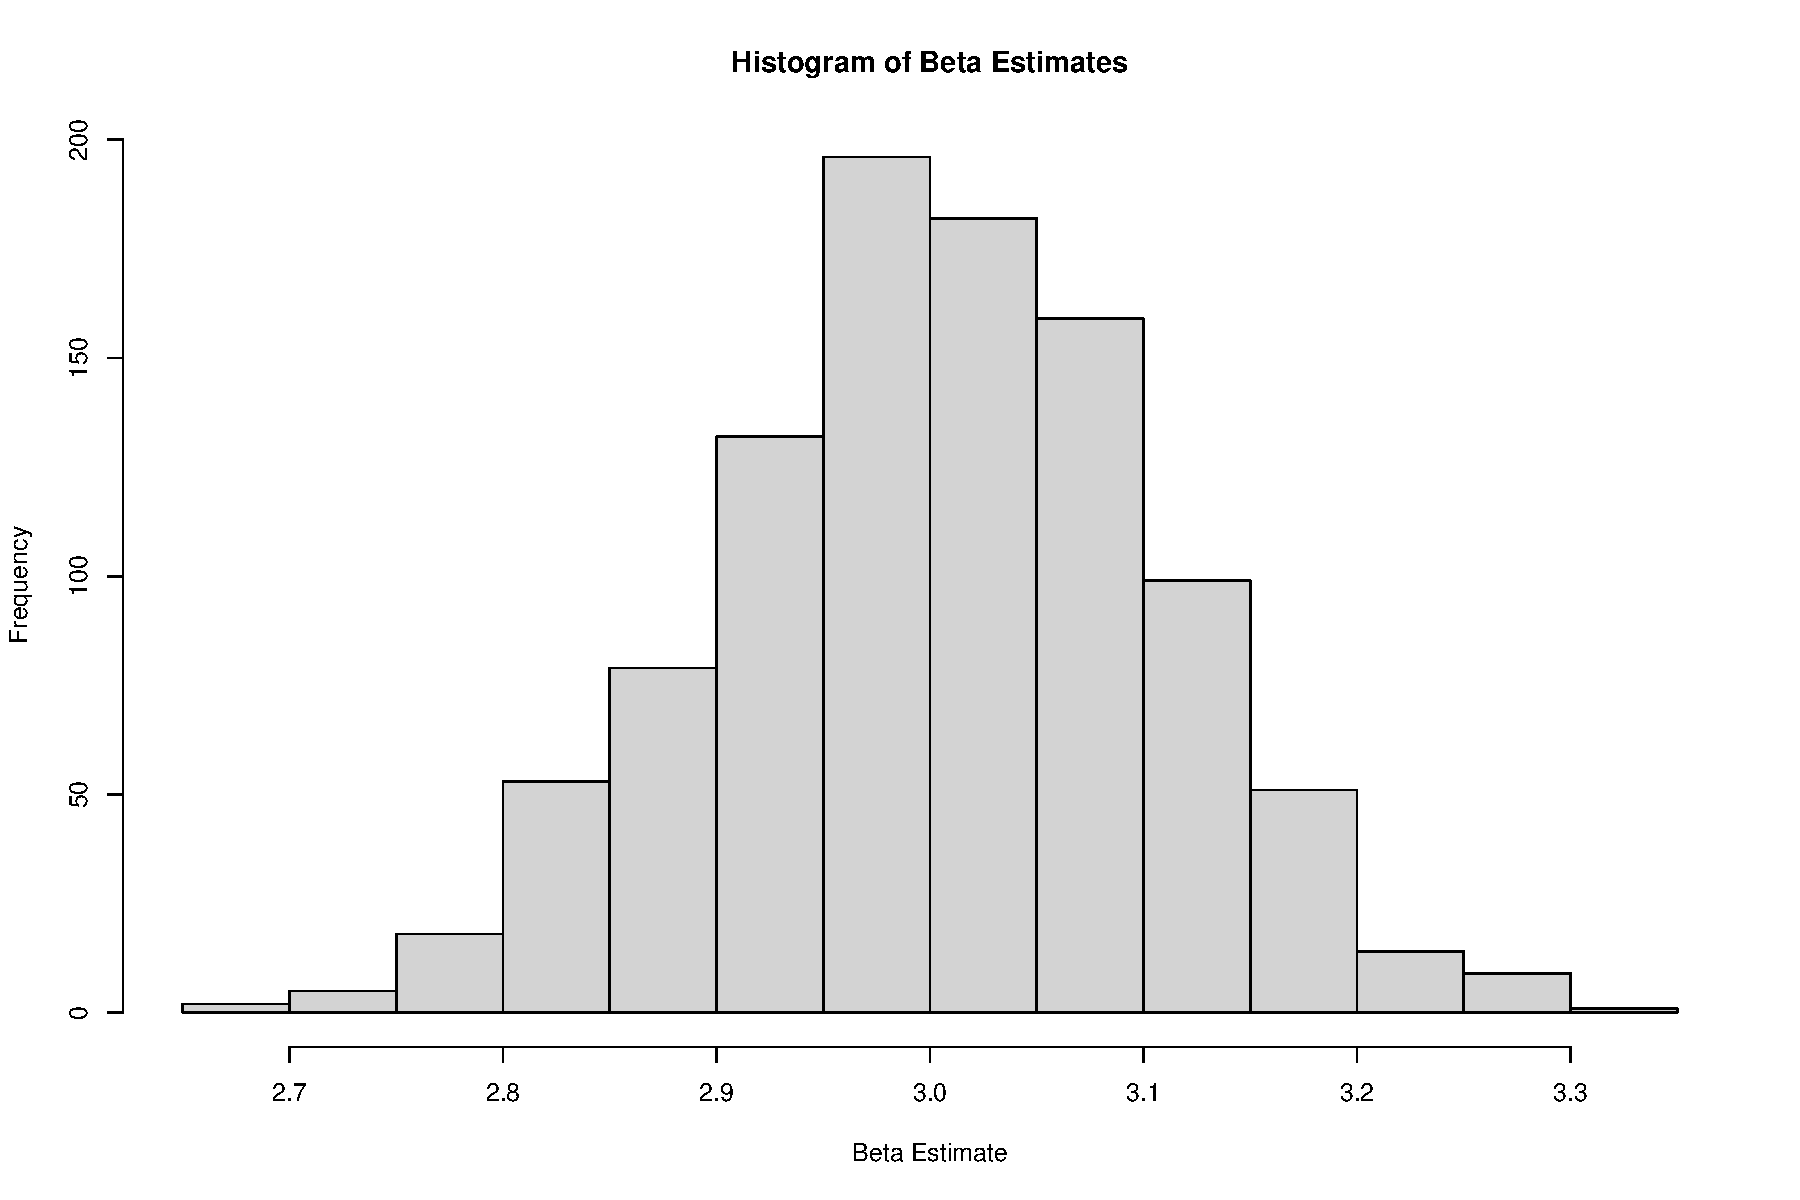
\includegraphics{Figures and Plots/figure-latex/global_options4-2.pdf} 

The approximately normal distribution of the beta\_lse estimates and its
central tendency around the true value of the slope coefficient of 3
suggests that the beta estimate is consistent. This means that as the
number of simulations approaches infinity, the estimates produced by the
estimator will converge to the true population value of the slope
coefficient, and the distribution of estimates will become increasingly
concentrated around the true value.
\vspace{2em}



\begin{center}
\textbf{Latent Variables}
\end{center}
\vspace{2em}

Latent variables are variables that can only be inferred indirectly from
other observable variables that can be directly observed or measured. 
As we know sigma, the latent values of the model in this case are the intercept and beta coefficient. These values are the true parameters that generate the data,
but they cannot be directly observed or measured. Instead, they are
estimated from the observed data.
\vspace{2em}


\begin{center}
\textbf{(very) Interesting research question}
\end{center}
\vspace{2em}

One potentially interesting regression to run could be to investigate
the relationship between a person's level of physical activity and their
self-reported levels of happiness. We could use a prior distribution to
specify our beliefs about the coefficient of interest, beta, before
observing any data. For example, we may specify a prior distribution
that assigns higher probability to positive values of beta, based on our
a priori expectation that physical activity is likely to have a positive
effect on happiness. We can then update our beliefs about beta after
observing the data, using Bayes' theorem to obtain the posterior
distribution of beta.

The posterior distribution of beta represents our updated beliefs about
the coefficient after observing the data, taking into account both the
prior distribution and the likelihood of the data given the model. The
posterior distribution can be used to make inferences about the
relationship between physical activity and happiness, such as the
probability that the coefficient of physical activity is positive or
negative, or the range of plausible values for the coefficient.

We will now implement a Bayesian analysis of the relationship between
physical activity and happiness. We are interested in the relationship between a person's level of
physical activity and their self-reported levels of happiness. To
incorporate our prior beliefs about this relationship, we set a positive
prior on the slope coefficient beta. The mean of the prior distribution
is set to 1, indicating that we believe physical activity is likely to
have a positive effect on happiness, while the standard deviation of the
prior distribution is set to 2, indicating that we allow for a wide
range of plausible values for the slope coefficient beta.

\vspace{2em}

\begin{Shaded}
\begin{Highlighting}[]
\NormalTok{knitr}\SpecialCharTok{::}\NormalTok{opts\_chunk}\SpecialCharTok{$}\FunctionTok{set}\NormalTok{(}\AttributeTok{fig.width=}\DecValTok{12}\NormalTok{, }\AttributeTok{fig.height=}\DecValTok{8}\NormalTok{, }\AttributeTok{fig\_path=}\StringTok{\textquotesingle{}figures/\textquotesingle{}}\NormalTok{,}\AttributeTok{echo=}\ConstantTok{TRUE}\NormalTok{, }\AttributeTok{warning=}\ConstantTok{FALSE}\NormalTok{, }\AttributeTok{message=}\ConstantTok{FALSE}\NormalTok{)}

\FunctionTok{library}\NormalTok{(MASS)  }\CommentTok{\# for the mvrnorm function}

\CommentTok{\# Define function to simulate data}
\NormalTok{sim\_linear\_model\_prior }\OtherTok{\textless{}{-}} \ControlFlowTok{function}\NormalTok{(n, k, alpha, beta\_prior\_mean, beta\_prior\_sd, sigma) \{}
\NormalTok{  X }\OtherTok{\textless{}{-}} \FunctionTok{matrix}\NormalTok{(}\FunctionTok{rnorm}\NormalTok{(n }\SpecialCharTok{*}\NormalTok{ k, }\AttributeTok{mean =} \DecValTok{0}\NormalTok{, }\AttributeTok{sd =} \DecValTok{1}\NormalTok{), n, k)}
\NormalTok{  beta }\OtherTok{\textless{}{-}} \FunctionTok{rnorm}\NormalTok{(k, }\AttributeTok{mean =}\NormalTok{ beta\_prior\_mean, }\AttributeTok{sd =}\NormalTok{ beta\_prior\_sd)}
\NormalTok{  epsilon }\OtherTok{\textless{}{-}} \FunctionTok{rnorm}\NormalTok{(n, }\AttributeTok{mean =} \DecValTok{0}\NormalTok{, }\AttributeTok{sd =}\NormalTok{ sigma)}
\NormalTok{  y }\OtherTok{\textless{}{-}}\NormalTok{ alpha }\SpecialCharTok{+}\NormalTok{ X }\SpecialCharTok{\%*\%}\NormalTok{ beta }\SpecialCharTok{+}\NormalTok{ epsilon}
  \FunctionTok{return}\NormalTok{(}\FunctionTok{list}\NormalTok{(}\AttributeTok{X =}\NormalTok{ X, }\AttributeTok{y =}\NormalTok{ y))}
\NormalTok{\}}

\CommentTok{\# Set seed for reproducibility}
\FunctionTok{set.seed}\NormalTok{(}\DecValTok{123}\NormalTok{)}

\CommentTok{\# Set prior parameters mu\_0 and sigma\_0}
\NormalTok{mu\_0 }\OtherTok{\textless{}{-}} \DecValTok{1}
\NormalTok{sigma\_0 }\OtherTok{\textless{}{-}} \DecValTok{2}

\CommentTok{\# Compute posterior for n = 50, 100, and 200}
\ControlFlowTok{for}\NormalTok{ (n }\ControlFlowTok{in} \FunctionTok{c}\NormalTok{(}\DecValTok{50}\NormalTok{, }\DecValTok{100}\NormalTok{, }\DecValTok{200}\NormalTok{)) \{}
  
  \CommentTok{\# Simulate data using sim\_linear\_model\_prior()}
\NormalTok{  k }\OtherTok{\textless{}{-}} \DecValTok{1}
\NormalTok{  alpha }\OtherTok{\textless{}{-}} \DecValTok{0}
\NormalTok{  beta\_prior\_mean }\OtherTok{\textless{}{-}} \DecValTok{0}
\NormalTok{  beta\_prior\_sd }\OtherTok{\textless{}{-}} \DecValTok{1}
\NormalTok{  sigma }\OtherTok{\textless{}{-}} \DecValTok{1}
  
\NormalTok{  sim\_data }\OtherTok{\textless{}{-}} \FunctionTok{sim\_linear\_model\_prior}\NormalTok{(n, k, alpha, beta\_prior\_mean, beta\_prior\_sd, sigma)}
\NormalTok{  X }\OtherTok{\textless{}{-}}\NormalTok{ sim\_data}\SpecialCharTok{$}\NormalTok{X}
\NormalTok{  y }\OtherTok{\textless{}{-}}\NormalTok{ sim\_data}\SpecialCharTok{$}\NormalTok{y}
  
  \CommentTok{\# Compute posterior parameters}
\NormalTok{  sigma\_n }\OtherTok{\textless{}{-}} \FunctionTok{solve}\NormalTok{(sigma\_0}\SpecialCharTok{\^{}}\NormalTok{(}\SpecialCharTok{{-}}\DecValTok{1}\NormalTok{) }\SpecialCharTok{+} \FunctionTok{t}\NormalTok{(X) }\SpecialCharTok{\%*\%}\NormalTok{ X)}
\NormalTok{  mu\_n }\OtherTok{\textless{}{-}}\NormalTok{ sigma\_n }\SpecialCharTok{\%*\%}\NormalTok{ (sigma\_0}\SpecialCharTok{\^{}}\NormalTok{(}\SpecialCharTok{{-}}\DecValTok{1}\NormalTok{) }\SpecialCharTok{*}\NormalTok{ mu\_0 }\SpecialCharTok{+} \FunctionTok{t}\NormalTok{(X) }\SpecialCharTok{\%*\%}\NormalTok{ y)}
  
  \CommentTok{\# Plot posterior density}
\NormalTok{  x\_grid }\OtherTok{\textless{}{-}} \FunctionTok{seq}\NormalTok{(}\SpecialCharTok{{-}}\DecValTok{5}\NormalTok{, }\DecValTok{5}\NormalTok{, }\AttributeTok{length.out =} \DecValTok{1000}\NormalTok{)}
\NormalTok{  post\_dens }\OtherTok{\textless{}{-}} \FunctionTok{dnorm}\NormalTok{(x\_grid, }\AttributeTok{mean =}\NormalTok{ mu\_n, }\AttributeTok{sd =} \FunctionTok{sqrt}\NormalTok{(sigma\_n))}
  \FunctionTok{plot}\NormalTok{(x\_grid, post\_dens, }\AttributeTok{type =} \StringTok{"l"}\NormalTok{, }\AttributeTok{lwd =} \DecValTok{2}\NormalTok{, }\AttributeTok{main =} \FunctionTok{paste0}\NormalTok{(}\StringTok{"Posterior Density (n = "}\NormalTok{, n, 
  }\StringTok{")"}\NormalTok{))}
\NormalTok{\}}
\end{Highlighting}
\end{Shaded}

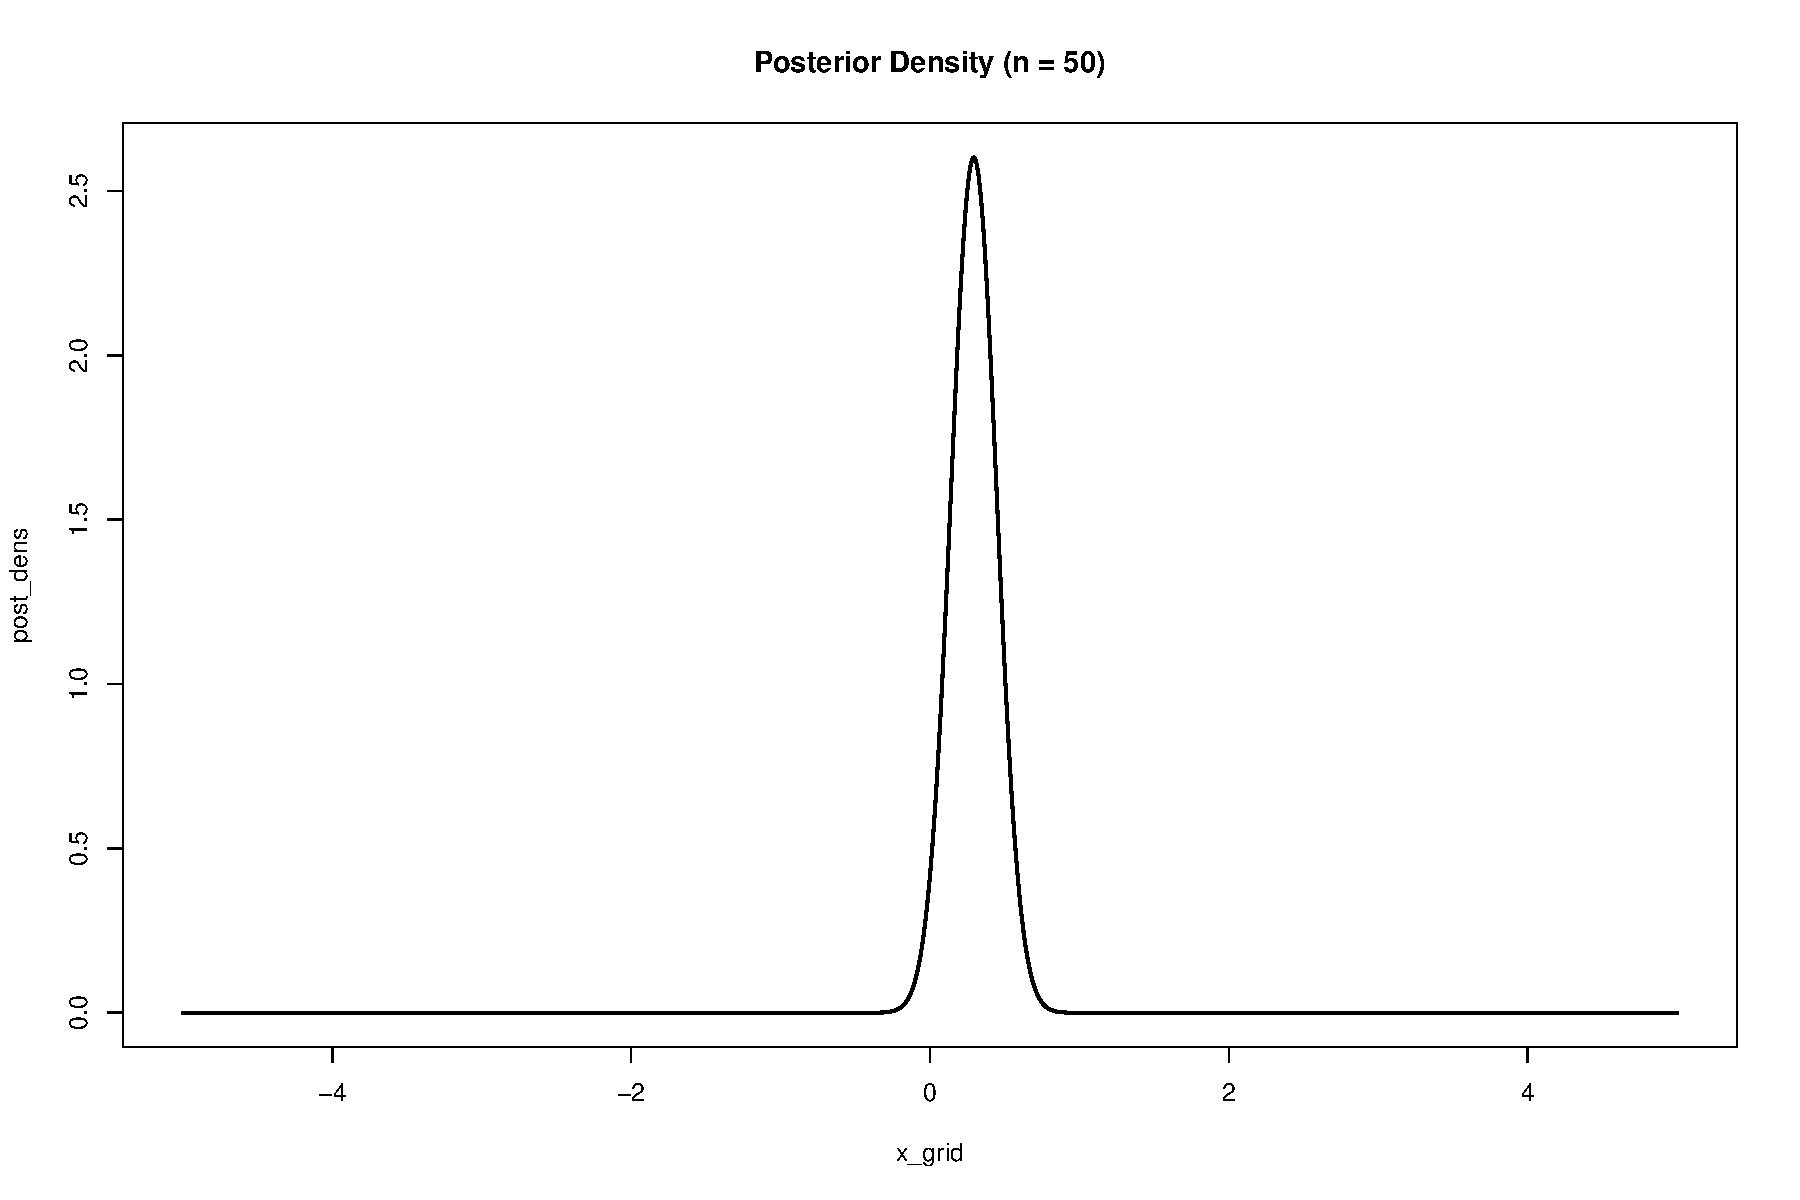
\includegraphics{Figures and Plots/figure-latex/global_options5-1.pdf}
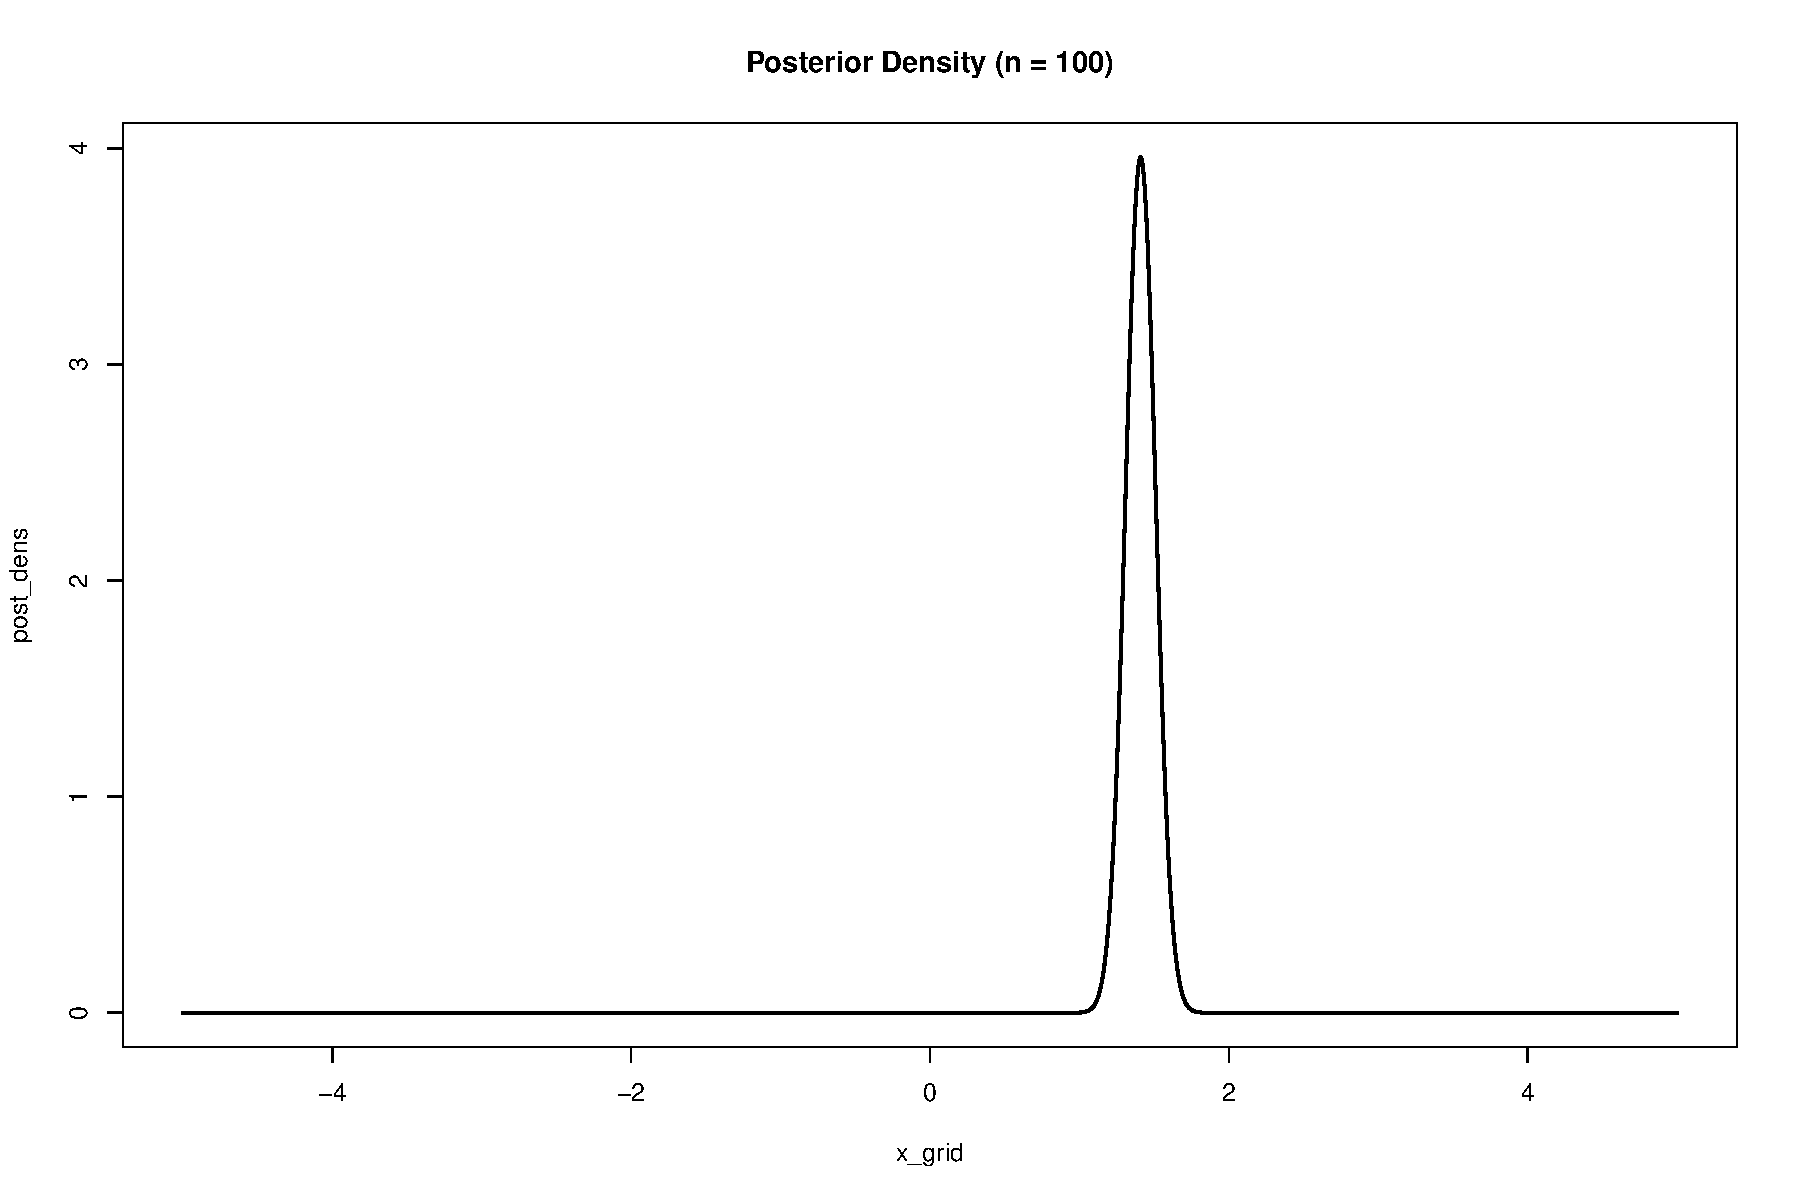
\includegraphics{Figures and Plots/figure-latex/global_options5-2.pdf}
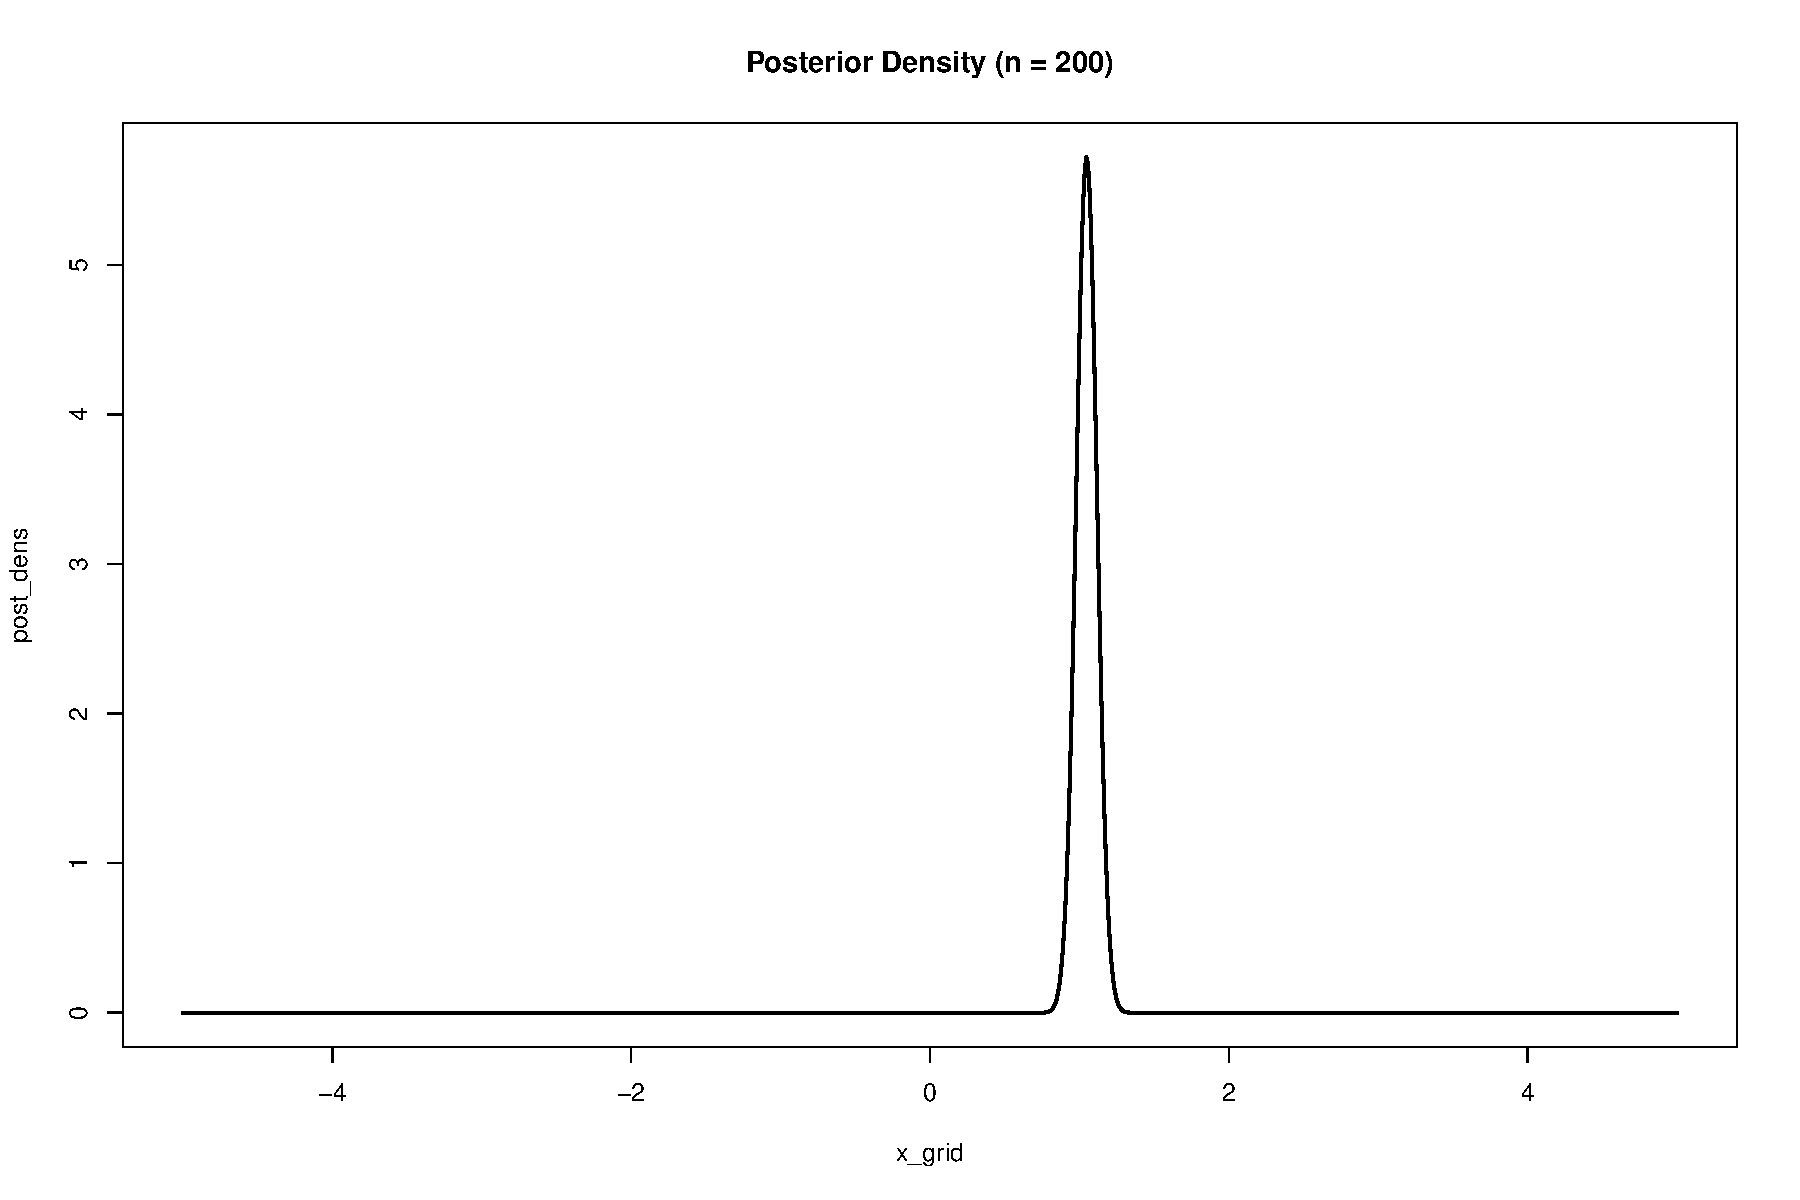
\includegraphics{Figures and Plots/figure-latex/global_options5-3.pdf}

The plots of the posterior density, given different sample sizes, show
that, as the sample size increases, the posterior density becomes more
concentrated around the true value of the slope parameters.
Additionally, as the sample size increases, the posterior density
becomes narrower, indicating that the uncertainty in the posterior
estimate decreases.

\section{Question 4}
\vspace{2em}


\begin{center}
\textbf{Known $\sigma^{2}$}
\end{center}
\vspace{2em}


The data are normally distributed: $y\sim N(\mu,1)$.
The prior is normal: $\mu \sim N(\mu_{0},\sigma_{0}^{2})$. Thus, the posterior is also normal.

We derive the posterior using Bayes' Theorem. The posterior distribution is proportional to the product of the likelihood and the prior. 

\begin{align*}
 p(\mu|y,\sigma^{2}) \propto p(y|\mu,\sigma^{2})*p(\mu|\sigma^{2})
\end{align*}   
\newpage

\textbf{Likelihood:} $y\sim N(\mu,1)$

\begin{align*}
    p(y|\mu,\sigma^{2})=\prod_{i=1}^{n}p(y_{i}|\mu,\sigma^{2})=(2\pi\sigma^{2})^{-n/2}\exp(-\frac{1}{2\sigma^{2}}\sum_{i=1}^{n}(y_{i}-\mu)^{2})
\end{align*}

We drop constant values that do not depend on $\mu$.

\begin{align*}
    p(y|\mu,\sigma^{2}) \propto \exp(-\frac{1}{2\sigma^{2}}\sum_{i=1}^{n}(y_{i}-\mu)^{2})
\end{align*}

We insert the variance decomposition $\sum_{i=1}^{n}(y_{i}-\mu)^{2}=n(\mu-\Bar{y})^{2}+(n-1)s^{2}$ that we proved in class after dropping constant values that don't depend on $\mu$.

\begin{align*}
    p(y|\mu,\sigma^{2}) \propto \exp(-\frac{(\mu-\Bar{y})^{2}}{2\sigma^{2}/n})
\end{align*}

\textbf{Prior:} $\mu \sim N(\mu_{0},\sigma_{0}^{2})$

\begin{align*}
    p(\mu|\mu_{0},\sigma_{0}^{2})=(2\pi\sigma^{2})^{-1/2}\exp(-\frac{1}{2\sigma_{0}^{2}}(\mu-\mu_{0})^{2}) \\ \propto \exp(-\frac{(\mu-\mu_{0})^{2}}{2\sigma_{0}^{2}})
\end{align*}

\textbf{Posterior:} $p(\mu|y,\sigma^{2}) \sim N(\mu_{n},\sigma_{n}^{2})$

\begin{align*}
    p(\mu|y,\sigma^{2}) \propto \exp(-\frac{(\mu-\mu_{0})^{2}}{2\sigma_{0}^{2}})\exp(-\frac{(\mu-\Bar{y})^{2}}{2\sigma^{2}/n}) \\
    =\exp(-\frac{1}{2\sigma_{0}^{2}}(\mu-\mu_{0})^{2})\exp(-\frac{n}{2\sigma^{2}}(\mu-\Bar{y})^{2}) \\
    =\exp(-\frac{1}{2\sigma_{0}^{2}}(\mu^{2}-2\mu_{0}\mu+\mu_{0}^{2})-\frac{n}{2\sigma^{2}}(\mu-2\Bar{y}\mu+\Bar{y}^{2}))\\
    =\exp(-\frac{1}{2}(\mu^{2}(\frac{1}{\sigma_{0}^{2}}+\frac{n}{\sigma^{2}})-2\mu(\frac{\mu_{0}}{\sigma_{0}^{2}}+\frac{n\Bar{y}}{\sigma^{2}})+\frac{\mu_{0}^{2}}{\sigma_{0}^{2}}+\frac{\Bar{y^{2}}}{\sigma^{2}}))
\end{align*}

We expect a normal posterior proportional to the following form:

\begin{align*}
    \exp(-\frac{1}{2\sigma_{n}^{2}}(\mu^{2}+\mu_{n}^{2}-2\mu\mu_{n}))
\end{align*}
\newpage
So, we need to match moments.

\begin{align*}
    -\frac{1}{2\sigma_{n}^{2}}\mu^{2}=-\frac{\mu^{2}}{2}(\frac{1}{\sigma_{0}}+\frac{n}{\sigma^{2}})\\
    \frac{1}{\sigma_{n}^{2}}=\frac{1}{\sigma_{0}^{2}}+\frac{n}{\sigma^{2}} \\
    \frac{1}{\sigma_{n}^{2}}=\frac{\sigma^{2}+\sigma_{0}^{2}n}{\sigma^{2}\sigma_{0}^{2}} \\
    \sigma_{n}^{2}=\frac{\sigma^{2}\sigma_{0}^{2}}{\sigma^{2}+\sigma_{0}^{2}n}
\end{align*}

The precision of the posterior is is equal to the sum of the precision of the prior and the data.

\begin{align*}
    \frac{2\mu\mu_{n}}{2\sigma^{2}_{n}}=\frac{\mu\mu_{n}}{\sigma^{2}_{n}}=\mu(\frac{\mu_{0}}{\sigma_{0}^{2}}+\frac{n\Bar{y}}{\sigma^{2}}) \\
    \frac{\mu_{n}}{\sigma^{2}_{n}}=\frac{\mu_{0}\sigma^{2}+n\Bar{y}\sigma_{0}^{2}}{\sigma_{0}^{2}\sigma^{2}} \\
    \mu_{n}=\sigma_{n}^{2}(\frac{\mu_{0}\sigma^{2}+n\Bar{y}\sigma_{0}^{2}}{\sigma_{0}^{2}\sigma^{2}})=\frac{\sigma_{0}^{2}\sigma^{2}}{\sigma^{2}+\sigma_{0}^{2}n}\frac{\mu_{0}\sigma^{2}+n\Bar{y}\sigma_{0}^{2}}{\sigma_{0}^{2}\sigma^{2}} \\
    =\frac{\mu_{0}\sigma^{2}+n\Bar{y}\sigma_{0}^{2}}{\sigma^{2}+\sigma_{0}^{2}n}
\end{align*}

Thus, the posterior follows the normal distribution: $p(\mu|y,\sigma^{2}) \sim N(\mu_{n},\sigma_{n}^{2})$, where $\mu_{n}=\frac{\mu_{0}+n\Bar{y}\sigma_{0}^{2}}{1+\sigma_{0}^{2}n}$ and $\sigma_{n}^{2}=\frac{\sigma_{0}^{2}}{1+\sigma_{0}^{2}n}$.

Below, we plot the histograms when using priors $\mu_{0}=0$ and $\sigma_{0}^{2}=1$ as well as $\mu_{0}=2$ and $\sigma_{0}^{2}=0.5$, respectively. 

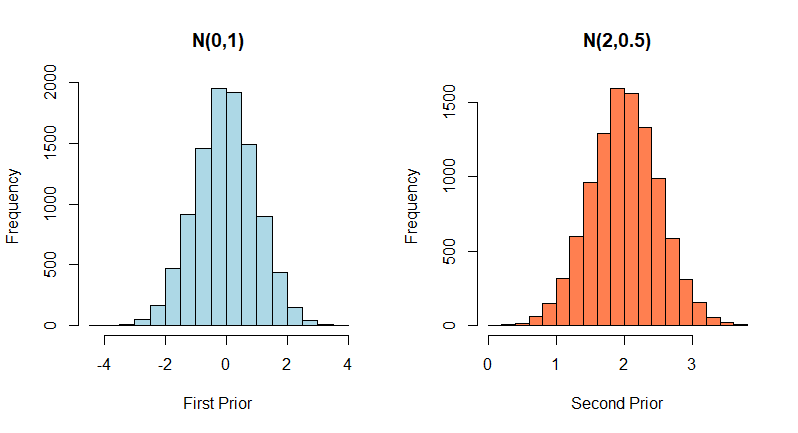
\includegraphics{Figures and Plots/figure-latex/Rplot 41.png}

\begin{center}
\textbf{Known $\mu$}
\end{center}
\vspace{2em}

The data are normally distributed: $y\sim N(5,\sigma^{2})$.
The prior for precision follows the Gamma distribution: $\sigma^{2} \sim G(0.5,\eta)$. The posterior for the precision then also follows the Gamma distribution, or equivalently, $\sigma^{2}$ follows the inverted Gamma distribution.

\textbf{Likelihood:} $y\sim N(5,\sigma^{2})$

Let $\tau=\sigma^{-2}$.

\begin{align*}
    p(y|\sigma^{2},\mu)=\prod_{i=1}^{n}p(y_{i}|\mu,\sigma^{2}) \\
    = (2\pi\sigma^{2})^{-n/2}\exp(-\frac{1}{2\sigma^{2}}\sum_{i=1}^{n}(y_{i}-\mu)/2)
\end{align*}

We drop constant values that don't depend on $\sigma^{2}$.

\begin{align*}
    p(y|\sigma^{2},\mu)\propto
    (\sigma^{2})^{-n/2+1-1}\exp(-\frac{1}{\sigma^{2}}\sum_{i=1}^{n}(y_{i}-\mu)/2) \\
    p(y|\tau,\mu)\propto
    \tau^{n/2+1-1}\exp(-\tau\sum_{i=1}^{n}(y_{i}-\mu)/2)
\end{align*}

The likelihood is proportional to the Gamma distribution $G(c,d)$ with shape parameter $c=-n/2+1$ and scale parameter $d=\sum_{i=1}^{n}(y_{i}-\mu)^{2}/2$.

\textbf{Prior:} $\sigma^{2} \sim G(0.5,\eta)$

\begin{align*}
    p(\tau|\eta)=\frac{\eta^{0.5}}{\Gamma(0.5)}\tau^{-0.5}\exp(-\eta\tau)
\end{align*}

We drop constant values that don't depend on $\tau$.

\begin{align*}
    p(\tau|\eta)\propto\tau^{-0.5}\exp(-\eta\tau)
\end{align*}

\textbf{Posterior:} $p(\tau|y,\mu)\sim G(c_{n},d_{n})$

\begin{align*}
    p(\tau|y,\mu) \propto p(y|\mu,\tau)p(\tau|\eta) \\
    =\tau^{n/2+1-1}\exp(-\tau\sum_{i=1}^{n}(y_{i}-\mu)^{2}/2)\tau^{-0.5}\exp(-\eta\tau) \\
    =\tau^{n/2+1-1}\exp(-\tau\sum_{i=1}^{n}(y_{i}-\mu)^{2}/2)\tau^{-0.5}\exp(-\eta\tau) \\
    = \tau^{n/2+0.5-1}\exp(-\tau\sum_{i=1}^{n}(y_{i}-\mu)^2/2-\eta\tau) \\
    = \tau^{\frac{n+1}{2}-1}\exp(-\tau(\eta+\sum_{i=1}^{n}(y_{i}-\mu)^2/2))
\end{align*}

Thus, the posterior follows the Gamma distribution $G(c_{n},d_{n})$ with shape parameter $c_{n}=\frac{n+1}{2}$ and scale parameter $d_{n}=\eta+\sum_{i=1}^{n}(y_{i}-5)^2/2$.

The prior density for $\eta \in {0.001,1,100}$ is displayed below.

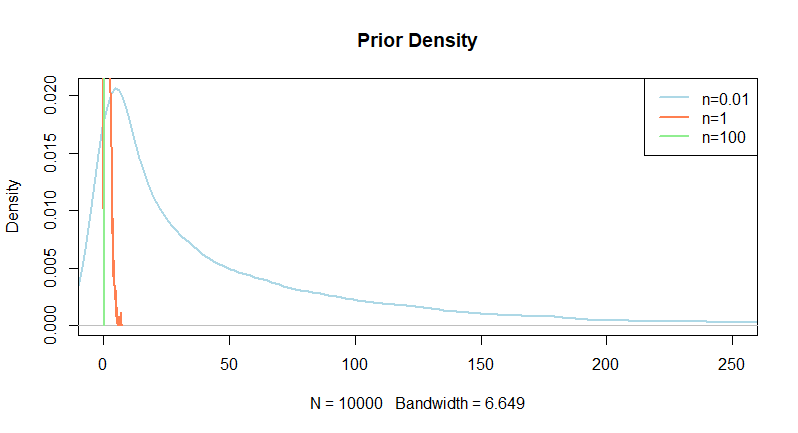
\includegraphics{Figures and Plots/figure-latex/Rplot 42.png}

\begin{center}
\textbf{Selection of hyperprior}
\end{center}

Since we are uncomfortable with choosing a value for $\eta$, we use a prior distribution. The prior for $\eta$ has to be positive. We could sample from the Gamma distribution since its support is the positive real line. Also, since it is a conjugate prior (as we have seen above), computation is facilitated. 

In our simulation, we draw $\eta$ from the Gamma distribution $G(5,5)$. We then draw priors for $\sigma^{2}$ from the Gamma distribution with shape parameter equal to 0.5 and simulated scale parameter $\eta$. The resulting density of $\sigma^{2}$ is displayed below. Problem: the graph for inverted gamma looks horrible, so I used the gamma distribution


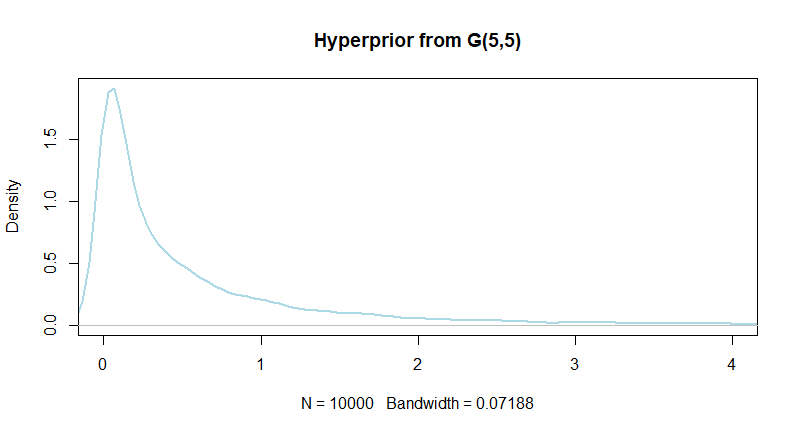
\includegraphics{Figures and Plots/figure-latex/Rplot 43.png}


\end{document}




